\documentclass[12pt]{report}

\newcommand\htmladdnormallink[2]{\href{#2}{#1}}

\textheight 22cm
\textwidth 15.5cm
\oddsidemargin 0pt\evensidemargin 0pt
%\oddsidemargin 14pt\evensidemargin 0pt
%\topmargin -40pt
\topmargin-30pt
%\bottommargin0pt
\def\baselinestretch{1.1}
%\addtolength{\parskip}{1ex}
\jot=.5ex
%\parskip = 0.02in


\setlength\arraycolsep{2pt}



\usepackage{amssymb}
\usepackage{amsmath,bm}
\usepackage{amssymb}
\usepackage{graphicx}
\graphicspath{ {../fig/} }
\usepackage{amsfonts}         
\usepackage{fancybox}   

%\usepackage[numbers]{natbib}

\usepackage{enumitem}

\usepackage{slashed}




\usepackage[usenames,dvipsnames]{xcolor}%http://en.wikibooks.org/wiki/LaTeX/Colors

\definecolor{darkgreen}{rgb}{0,0.4,0}
\definecolor{darkred}{rgb}{0.4,0,0}
\definecolor{darkblue}{rgb}{0,0,0.4}
\definecolor{lightblue}{rgb}{.6,.6,0.9}
\newcommand{\cobl}{\color{darkblue}}

\newcommand{\cor}{\color{red}}
\newcommand{\cog}{\color{darkgreen}}
\newcommand{\cob}{\color{black}}

\definecolor{uglybrown}{rgb}{0.8,  0.7,  0.5}

\def\ii{{\bf i}}
\def\Ione{\mathbb{I}}
\def\UU{{\bf U}}
\def\HH{{\bf H}}
\def\pp{{\bf p}}
\def\aa{{\bf a}}
\def\qq{{\bf q}}
\def\eps{\epsilon}
\def\half{{1\over 2}}
\def\Tr{{{\rm Tr~ }}}
\def\tr{{\rm tr}}
\def\Re{{\rm Re\hskip0.1em}}
\def\Im{{\rm Im\hskip0.1em}}
\def\ppi{\boldsymbol{\pi}}
\def\pphi{\boldsymbol{\phi}}
%\def\pphi{\phi}
\def\grad{\vec \nabla}
\def\vB{\vec B}
\def\vE{\vec E}
\def\vA{\vec A}
\def\vAA{ \vec{\bf A}}
\def\vEE{{{\vec {\bf E}}}}
\def\vBB{{\vec {\bf B}}}

\def\CL{{\cal L}}



\def\bra#1{\left\langle#1\right|}
\def\ket#1{\left|#1\right\rangle}
\def\bbra#1{{\langle\langle}#1|}
\def\kket#1{|#1\rangle\rangle}
\def\vev#1{\left\langle{#1}\right\rangle}

\def\ketbra#1#2{ | #1 \rangle\hskip-2pt\langle #2|}



\def\be{\begin{equation}}
\def\ee{\end{equation}}
\def\({\left(}
\def\){\right)}



\newcommand{\bea}{\begin{eqnarray}}
\newcommand{\eea}{\end{eqnarray}}


\def\parfig#1#2{
\parbox{#1\textwidth}
{\includegraphics[width=#1\textwidth]{#2}}
}



%%from  Rudro Rana Biswas
\usepackage[pagebackref,  % this puts links to the page numbers where refs appear
%pdftex, 
bookmarks={false}, pdfauthor={John McGreevy}, pdftitle={Yay, physics!}]{hyperref}
\hypersetup{colorlinks=true, 
linkcolor=BrickRed, 
citecolor=Violet, 
filecolor=OliveGreen, 
urlcolor=RoyalBlue, 
filebordercolor={.8 .8 1}, 
urlbordercolor={.8 .8 0}}%http://en.wikibooks.org/wiki/LaTeX/Hyperlinks


%\usepackage{mathtools} % for inclusion arrow \xhookrightarrow{}


\renewcommand{\theequation}{\arabic{equation}}
\newif{\ifeq}           % defines a new condition @eq tested by the conditional \ifeq
\eqtrue                 % if uncommented, declares @eq to be true
%\eqfalse              % if uncommented, declares @eq to be false
%                                %
%                                % to use this, wrap text with the conditional, eg:
%                                %
%                                % \ifeq
%                                % SHOW THIS IFF \eqtrue HAS BEEN DECLARED
%                                % \fi
%
\def\answer#1
{
\ifeq
\textcolor{darkblue}{#1}
\fi
}

\begin{document}
\begin{center}

University of California at San Diego -- 
Department of Physics --
Prof.~John McGreevy

{\Large\bf  Physics 210B Non-equilibrium  Fall 2025}\\
{\Large\bf Assignment 2 \answer{--~~~ Solutions} }
\end{center}


\noindent
\hfill {\bf Due 11:59pm {Monday, October 13, 2025}} 





\bigskip
\hrule




\begin{enumerate}



\item{\bf Brain-warmer: Optimal selection.}

%``In many specialized populations, there is little variability among the members.
%Is this a natural consequence of optimal selection?"
%For example, 
Take a gazillion random humans and break them into groups of $n$.
Make each group of $n$ race some fixed distance, say 26.2 miles, and record their average speed.
Normalize these results by the world record, which is (amazingly) 
${\text{26.2 miles}\over\text{2:00:35}}$
%$ {\text{26.2 miles}\over\text{2:03:59 = 123.98 minutes} }$ 
(held by the late Kelvin Kiptum  since 2023), so $r = {\text{speed} \over \text{world record speed} } \in [0,1]$.
(For people who don't make it the whole distance (for example because they are infants and can't walk yet) the result is $r=0$.)
Now suppose we select the largest result from each group of $n$, i.e.~the average speed of the winner of each race, and call it $x$.
What will be the distribution of values of $x$?  
If we pick $n$ big enough, so that we find an elite marathon runner in each group, we might expect that they are going to cluster pretty close together.

\answer{For small n, the distribution of x will be broad, but as n increases, the distribution will become more concentrated near 1, reflecting the selection of the fastest runners.}

\begin{enumerate}
\item Let $\{r_\alpha \}$ be $n$ random numbers, each independently chosen
from a probability density $p(r)$, with $r \in [0,1]$.  
Find the probability density $p_n(x)$ for 
the {\it largest} value in the set, i.e.~for 
$ x = \text{max}\{r_1, ... r_n \}$.

\answer{
\begin{equation}
p_n(x) = n p(x) \left( \int_0^x p(r') dr' \right)^{n-1}. 
\end{equation}}

\item Consider the special case where $p(r)$ is uniform on $[0,1]$.
Find $\vev{x}$ and $\text{Var}(x)$ for this case and think about what happens at large $n$.  
Does it agree with the expectation mentioned above?

\answer{
\begin{equation}
\vev{x} = \frac{n}{n+1}, \quad \text{Var}(x) = \frac{n}{(n+1)^2(n+2)}.
\end{equation}
As $n$ increases, $\vev{x}$ approaches 1, and $\text{Var}(x)$ decreases, indicating that the distribution becomes more concentrated near 1. This agrees with the expectation that elite runners cluster closely together.}

\end{enumerate}


\item {\bf Large deviation principle.} In this problem we will 
see whether the rate function $I(S)$ ($S \equiv \sum_{i=1}^N x_i^N/N$) computed by saddle point (i.e.~the large deviation principle)
agrees with the exact calculation for two examples of random walks.

\begin{enumerate}
\item {\bf Fixed-step-length with bias.} Consider a 1d random walk where each step has magnitude $1$ with probability $p$ for $x_i = +1$ and probability $1-p$ for $x_i = -1$.
Find the exact distribution $P_N(S)$ of the average displacement $S =  \sum_{i=1}^N x_i/N$ after $N$ steps and use Stirling's formula to write it in the form 
$ P_N(S) = f(S) e^{ - N I(S)}$.  

\answer{
\begin{equation}
S = \frac{1}{N} \sum_{i=1}^N x_i, \quad x_i = \pm 1, 
\end{equation}
Let K be the number of +1 steps, then the number of -1 steps is N-K. Thus,
\begin{equation}
S = \frac{K - (N-K)}{N} = \frac{2K - N}{N} \implies K = \frac{N(1+S)}{2}.
\end{equation}
The probability of getting K steps of +1 and N-K steps of -1 is given by the binomial distribution:
\begin{equation}
P_N(S) = \binom{N}{K} p^K (1-p)^{N-K} = \binom{N}{\frac{N(1+S)}{2}} p^{\frac{N(1+S)}{2}} (1-p)^{\frac{N(1-S)}{2}}.
\end{equation}
Using Stirling's approximation, we can express this in the form:
\begin{equation}
P_N(S) \approx f(S) e^{-N I(S)},
\end{equation}
where
\begin{equation}
I(S) = \frac{1+S}{2} \ln\left(\frac{1+S}{2p}\right) + \frac{1-S}{2} \ln\left(\frac{1-S}{2(1-p)}\right).
\end{equation}
} 

Now find the rate function by the method of large deviations and check that you get the same answer.

\answer{
\begin{equation}
S = \frac{1}{N} \sum_{i=1}^N x_i
\end{equation}
\begin{equation}
I(s) = \sup_{t \in \mathbb{R}} \left[ ts - \lambda(t) \right]
\end{equation}
\begin{equation}
\lambda(t) = \log \mathbb{E}\left[ e^{t x_1} \right] = \log \left( p e^{t} + (1-p) e^{-t} \right)
\end{equation}
\begin{equation}
\frac{d\lambda}{dt} = s
\end{equation}
\begin{equation}
\frac{p e^{t} - (1-p) e^{-t}}{p e^{t} + (1-p) e^{-t}} = s
\end{equation}
\begin{equation}
s = \frac{p y - (1-p)}{p y + (1-p)}
\end{equation}
let $y = e^{2t}$
\begin{equation}
y = \frac{(1-p)(1+s)}{p(1-s)}
\end{equation}
\begin{equation}
t^*(s) = \frac{1}{2} \log \left[ \frac{(1-p)(1+s)}{p(1-s)} \right]
\end{equation}
\begin{equation}
I(s) = t^*(s)\, s - \lambda\!\left( t^*(s) \right)
\end{equation}
\begin{equation}
q = \frac{1 + s}{2}, \qquad s = 2q - 1
\end{equation}
\begin{equation}
I(s) = q \ln \frac{q}{p} + (1 - q) \ln \frac{1 - q}{1 - p}
\end{equation}
\begin{equation}
I(s) = \frac{(s - (2p - 1))^2}{8 p (1 - p)} + \mathcal{O}\!\left( (s - (2p - 1))^3 \right)
\end{equation}}

\item {\bf Exponential distribution.}  Suppose now that each step is sampled from the exponential distribution,
\be P(x) = {1\over \mu} e^{ - x/\mu} , x \geq 0 . \ee
Find the exact distribution for the average displacement $S =  \sum_{i=1}^N x_i/N$ after $N$ steps 
and use Stirling's formula to write it in the form 
$ P_N(S) = f(S) e^{ - N I(S)}$.  

\answer{
\begin{equation}
P(x)=\frac{1}{\mu} e^{-x/\mu},\qquad x\ge 0
\end{equation}
\begin{equation}
S=\frac{1}{N}\sum_{i=1}^N x_i
\end{equation}
\begin{equation}
f_X(X)=\frac{1}{\mu^N \Gamma(N)}\,X^{N-1} e^{-X/\mu},\qquad X\ge 0
\end{equation}
\begin{equation}
P_N(S)=\frac{N^N}{\mu^N\Gamma(N)}\,S^{N-1}\,e^{-NS/\mu},\qquad S\ge 0
\end{equation}
\begin{equation}
\Gamma(N)\approx \sqrt{2\pi}\,N^{\,N-\frac{1}{2}} e^{-N}
\end{equation}
\begin{equation}
P_N(S)\approx \frac{\sqrt{N}}{\sqrt{2\pi}\,S}\,
\exp\!\left\{-N\!\left(\frac{S}{\mu}-1-\ln\frac{S}{\mu}\right)\right\}
\end{equation}
\begin{equation}
I(S)=\frac{S}{\mu}-1-\ln\frac{S}{\mu},\qquad S\ge 0
\end{equation}}


Now find the rate function by the method of large deviations.  Do you get the same answer?
\answer{
\begin{equation}
\lambda(t)=\log\mathbb{E}\big[e^{t x}\big]=-\log(1-\mu t),\qquad t<\frac{1}{\mu}
\end{equation}
\begin{equation}
I(S)=\sup_{t<1/\mu}\left[tS-\lambda(t)\right]
=\sup_t\left[tS+\log(1-\mu t)\right]
\end{equation}
\begin{equation}
S-\frac{\mu}{1-\mu t}=0 \quad\Longrightarrow\quad t^*=\frac{1}{\mu}-\frac{1}{S}
\end{equation}
\begin{equation}
I(S)=t^*S+\log(1-\mu t^*)
=\left(\frac{1}{\mu}-\frac{1}{S}\right)S+\log\!\frac{\mu}{S}
=\frac{S}{\mu}-1-\log\frac{S}{\mu}
\end{equation}
\begin{equation}
I(S)=\frac{(S-\mu)^2}{2\mu^2}+O\!\left((S-\mu)^3\right),\qquad
\mathrm{Var}(S)\approx \frac{\mu^2}{N}
\end{equation}}

\end{enumerate}

\item {\bf Tracy-Widom distribution.}  [Bonus problem]

Use the method of large deviations to derive the Tracy-Widom distribution for the largest eigenvalue of a (Gaussian) random (real, symmetric) matrix.




\item{\bf Gillespie algorithm or continuous-time Monte Carlo, and demographic stochasticity.}
Consider a `dimerization reaction': a molecule $M$ (`monomer') joins with another monomer to form a dimer $ 2 M \leftrightarrow D$.  The forward reaction rate is $k_d$ and the backwards rate is $k_u$.
That is, the backwards unbinding rate per unit volume is $k_u[D]$ 
(where $[D]$ is the concentration of dimers),
while the forward binding rate per unit volume is $k_b[M]^2$ (since the binding requires a collision of two monomers).  
[actually $ k_b M (M-1)$.]
For definiteness, let's take all $N$ monomers to be initially unbound, 
and $k_u = 2 k_b$. %[COMMENT ON UNITS.]




\begin{enumerate}
\item Write an ODE for $\partial_t M$ treating $M$ and $D$ as continuous variables.  

Find the equilibrium values of $[M]$ and $[D]$ for the given values of $k_u$ and $k_b$ for $N=2, 90, 10000$.  
Solve the ODE numerically and verify that the late time behavior agrees with the equilibrium solutions you found.
\answer{
\begin{equation}
\dot{M} = -2k_b M^2 + 2k_u D
\end{equation}
\begin{equation}
M + 2D = N
\end{equation}
\begin{equation}
-2k_b M^2 - k_u M + k_u N = 0
\end{equation}
\begin{equation}
M^* = \frac{-k_u + \sqrt{k_u^2 + 8 k_b k_u N}}{4k_b}
\end{equation}
\begin{equation}
M^* = \frac{-1 + \sqrt{1 + 8 r N}}{4r}, \qquad r \equiv \frac{k_b}{k_u}
\end{equation}
\begin{equation}
D^* = \frac{N - M^*}{2} = \frac{k_b}{k_u}\,(M^*)^2
\end{equation}
\begin{equation}
\text{For } k_b=1,\; k_u=2:\quad M^* = \frac{-1 + \sqrt{1 + 4N}}{2}
\end{equation}
\begin{equation}
D^* = \frac{N - M^*}{2}
\end{equation}
\begin{equation}
\text{For } N=2:\quad M^* = 1,\qquad D^* = 0.5
\end{equation}
\begin{equation}
\text{For } N=90:\quad M^* = 9,\qquad D^* = 40.5
\end{equation}
\begin{equation}
\text{For } N=10000:\quad M^* \approx 99.50125,\qquad D^* \approx 4950.2494
\end{equation}}
\end{enumerate}

When the number of molecules is small, we expect that the continuum approximation above may fail.  Here is an efficient Monte Carlo algorithm to simulate the individual molecule evolution.

Suppose that the reactions have rates $\Gamma_i$ with $ \Gamma_\text{tot} = \sum_i \Gamma_i$, so the probability that the next reaction that happens is reaction $j$ is $ \Gamma_j/\Gamma_\text{tot}$.  
To simulate until a final time $t_f$: 
Pick a random time $t_\text{wait}$ with probability distribution 
$p(t) = \Gamma_\text{tot} e^{ - \Gamma_\text{tot} t}$.  

If the current time $t$ plus $t_\text{wait}$ is bigger than $t_f$, you are done.

Otherwise, increment $t$ by $t_\text{wait}$, pick a random number $r$ uniformly in the interval $[0, \Gamma_\text{tot})$, and execute the reaction $j$ for which 
$ \sum_{i<j} \Gamma_i \leq r < \sum_{i< j + 1} \Gamma_i $, i.e.~such that $r$ lands in the $j$th interval of the sum forming $\Gamma_\text{tot}$.  

Repeat.  (If some reaction becomes impossible, you may need to recompute $\Gamma_\text{tot}$.)

\begin{enumerate}[resume]
\item Implement this algorithm for the dimerization reaction, and simulate for $N=2, 90, 10000$ and compare individual trajectories with the continuum solution.  
For what $N$ are the fluctuations at late times less than $\pm 20 \%$? 

\answer{
    \begin{figure}[h!]
    \centering
    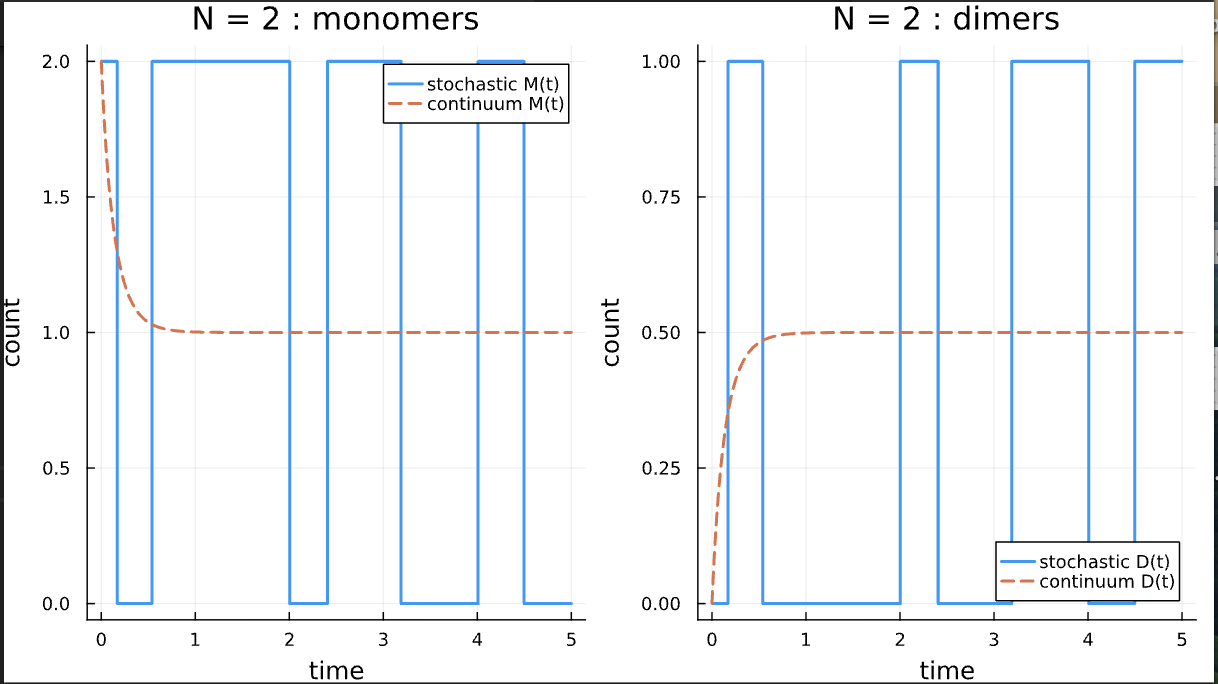
\includegraphics[width=0.8\textwidth]{n=2.png}
    \caption{Stochastic trajectory for N=2}
    \end{figure}
    \begin{figure}[h!]
    \centering
    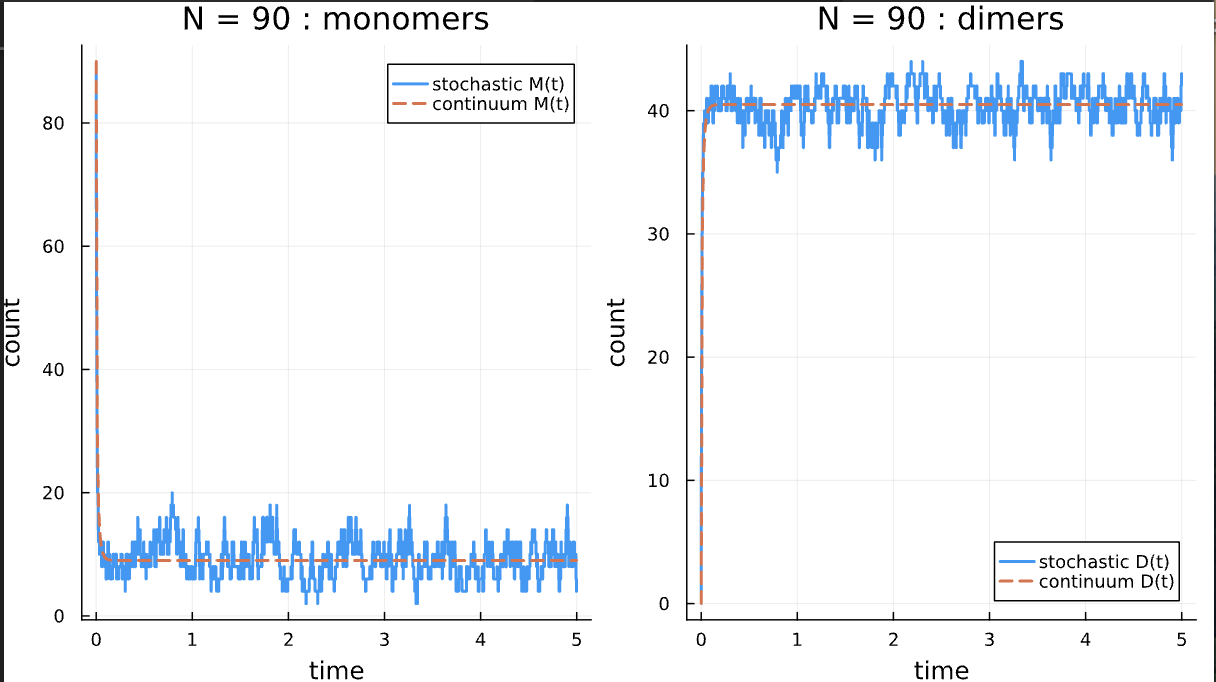
\includegraphics[width=0.8\textwidth]{n=90.png}
    \caption{Stochastic trajectory for N=90}
    \end{figure}
    \begin{figure}[h!]
    \centering
    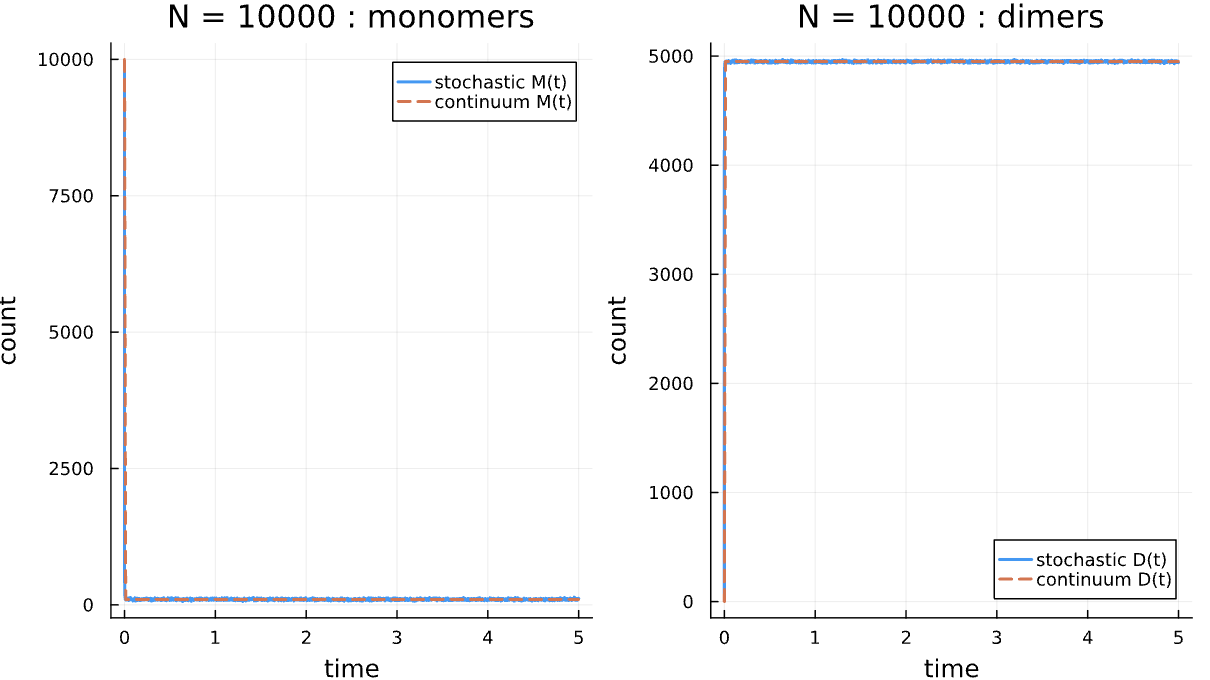
\includegraphics[width=0.8\textwidth]{n=10000.png}
    \caption{Stochastic trajectory for N=10000}
    \end{figure}
For N=10000, the fluctuations at late times are less than ±20 (See figure 1,2,3).
}

\item Find the average of many realizations of the discrete evolution for $N=2, 90$ and compare with the ODE result.  How much is the long-term average shifted by the demographic stochasticity?  
How large does $N$ need to be for the ensemble average of $M(t)$ to be well-described by the ODE? 

\answer{
    \begin{figure}
    \centering
    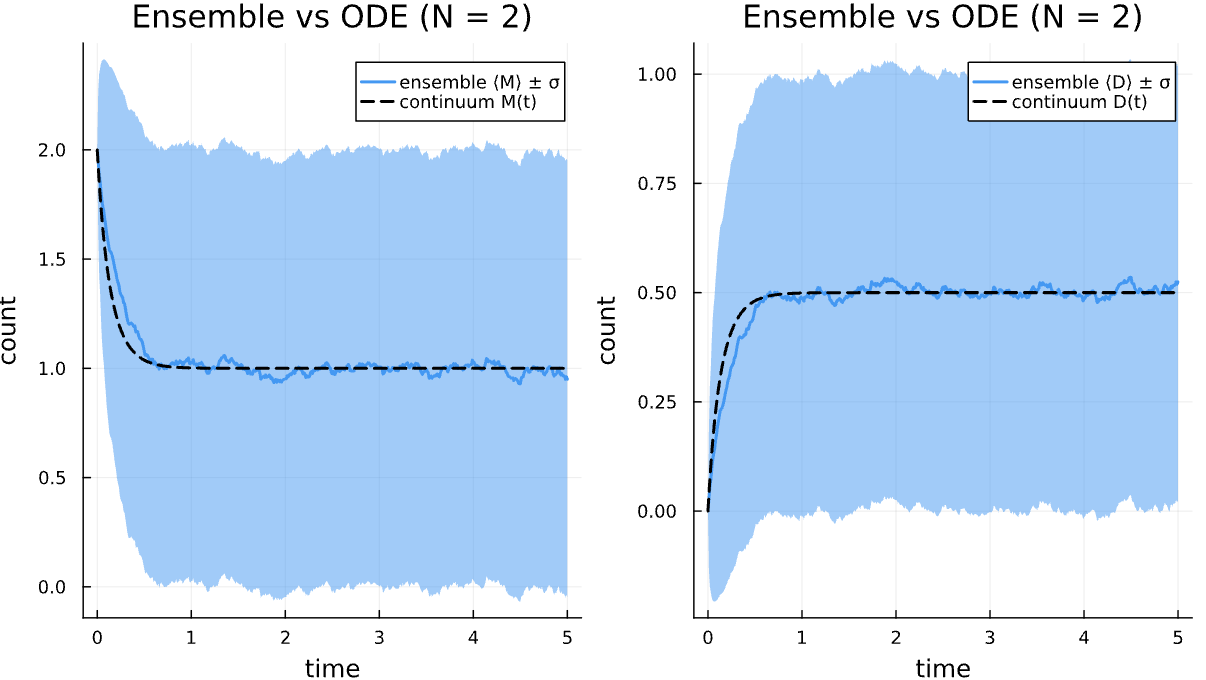
\includegraphics[width=0.8\textwidth]{averagen=2.png}
    \caption{Average of many realizations for N=2, compared with ODE result}
    \end{figure}
    \begin{figure}
    \centering
    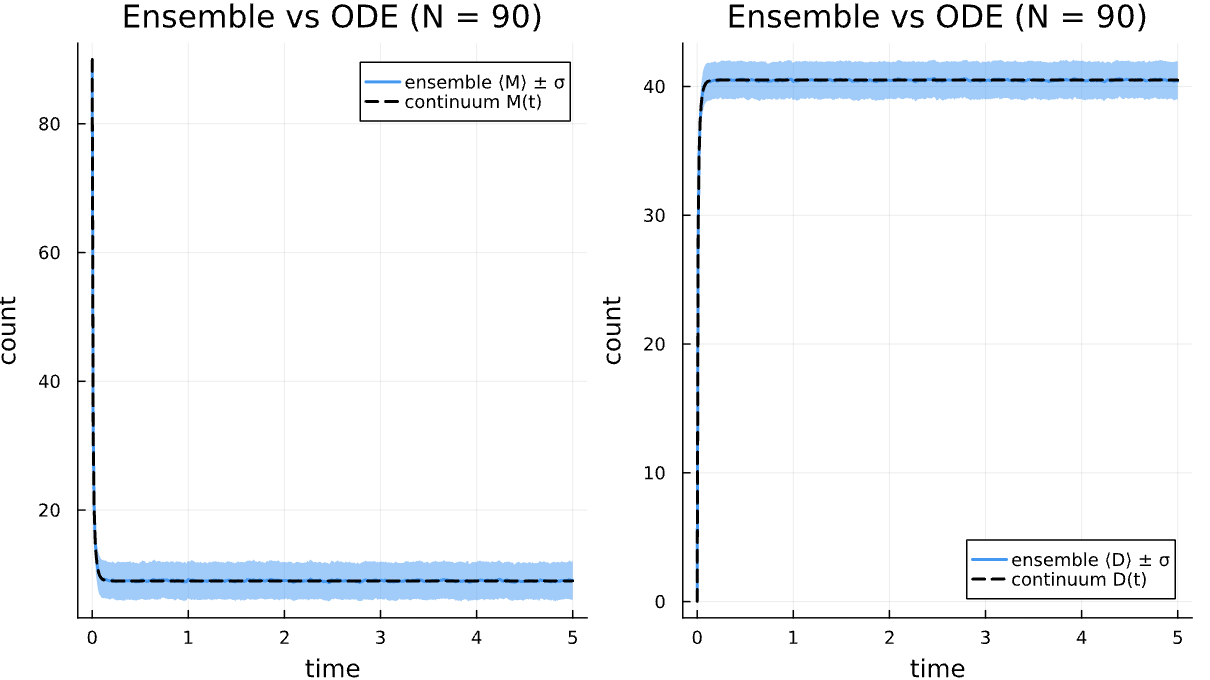
\includegraphics[width=0.8\textwidth]{averagen=90.png}
    \caption{Average of many realizations for N=90, compared with ODE result}
    \end{figure}
For N=90, the ensemble average of M(t) is well-described by the ODE (See figure 4,5). 
}


\item Use these ideas to simulate a 1d continuous-time random walk (CTRW) (say for a distribution $p_t(t)$ with a long tail) without actually waiting for the possibly-long waiting times.

\answer{
    Please see figure 6. 
    \begin{figure}
    \centering
    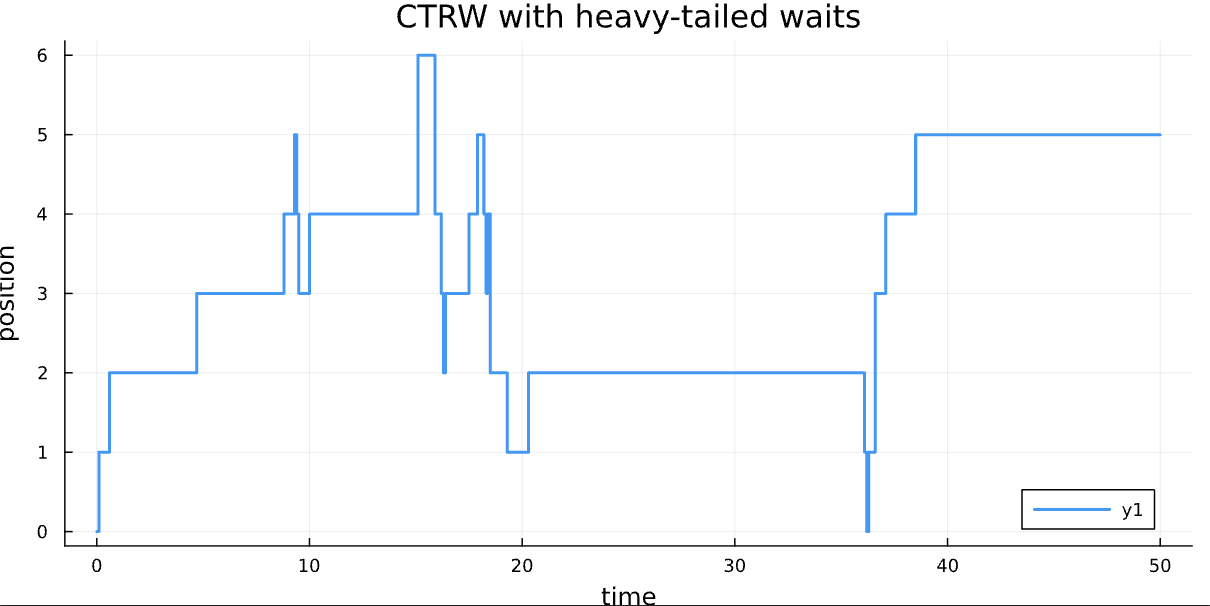
\includegraphics[width=0.8\textwidth]{ctrw.png}
    \caption{CTRW with heavy-tailed waits}
    \end{figure}
}

\end{enumerate}







\end{enumerate}
\end{document}
